\subsection{RQ1: per-token KV cost fell every year; per-parameter cost fell with a 2025 rebound}
\label{sec:rq1}

% AUTO-GENERATED by make analysis - do not edit by hand
\begin{table}[t]\centering\scriptsize\setlength{\tabcolsep}{3.5pt}
\caption{Census overview. Rows are checkpoints; family-dedup keeps one row per publisher family with identical geometry, geo-dedup one row per distinct attention geometry.}\label{tab:overview}
\begin{tabular}{lrrrrrrr}\toprule
year & rows & family & geo & med.\ KV/tok & IQR & B/tok/$10^9$p & geo B/tok/$10^9$p\\\midrule
2023 & 263 & 243 & 50 & 327680 & 487424 & 72087.7 & 61170.6\\
2024 & 670 & 563 & 78 & 131072 & 240640 & 25720.2 & 14800.3\\
2025 & 1044 & 949 & 104 & 70272 & 172032 & 76468.6 & 9238.2\\
2026 & 354 & 313 & 60 & 36864 & 135168 & 7374.3 & 861.7\\
\bottomrule\end{tabular}\end{table}


\begin{figure}[t]
\centering
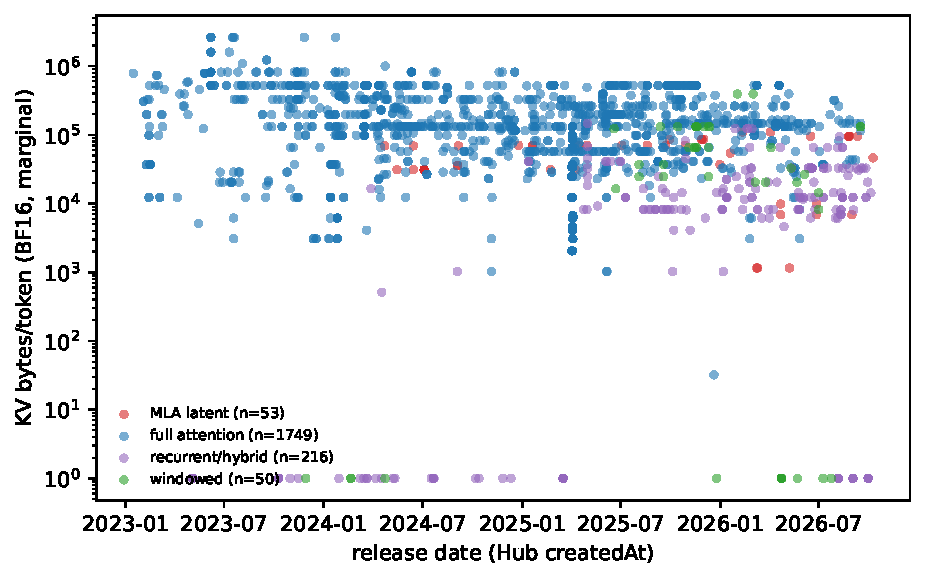
\includegraphics[width=.8\linewidth]{figures/fig1_kv_trend.pdf}
\caption{Marginal KV bytes per token (BF16) against release date for the deduplicated census, log-scale $y$ axis; color encodes the coarse attention class.}
\label{fig:kv-trend}
\end{figure}

Table~\ref{tab:overview} and Figure~\ref{fig:kv-trend} summarize the deduplicated census of \kvcDedupRows{} geometry groups. The median marginal KV cost in BF16 fell in every release year: \kvcMedianKvTokTwentyThree{} bytes per token in 2023, \kvcMedianKvTokTwentyFour{} in 2024, \kvcMedianKvTokTwentyFive{} in 2025, and \kvcMedianKvTokTwentySix{} in 2026. Spearman rank correlations against release date confirm a decline on both outcomes: $\rho=\kvcSpearmanRho$ ($p=\kvcSpearmanP$) for KV bytes per token and $\rho=\kvcSpearmanRhoPP$ ($p=\kvcSpearmanPPp$) for KV per parameter. The correlations are weak in magnitude because the within-year spread dwarfs the between-year shift; in Figure~\ref{fig:kv-trend} the full-attention, windowed, recurrent/hybrid, and MLA-latent classes overlap across orders of magnitude at every date. The decline tracks the diffusion of cost-saving designs rather than a single event: KV-head reduction cuts the per-token cost at fixed width \cite{shazeer2019mqa,ainslie2023gqa}, sliding-window layers bound the cache \cite{jiang2023mistral}, and latent compression shrinks it further \cite{deepseekai2024v2}; Figure~\ref{fig:kv-trend} shows windowed and recurrent/hybrid points becoming denser at later dates.

The per-parameter picture is not monotone. Median KV bytes per token per $10^{9}$ parameters dropped from \kvcMedianKvppTwentyThree{} in 2023 to \kvcMedianKvppTwentyFour{} in 2024, rebounded to \kvcMedianKvppTwentyFive{} in 2025---above the 2023 level---and then fell to \kvcMedianKvppTwentySix{} in 2026. We read the rebound as a release-mix effect rather than an architectural regression. The 2025 cohort contributes \kvcRqOneNTwentyFive{} of the \kvcDedupRows{} deduplicated groups, against \kvcRqOneNTwentyThree{} in 2023 (Table~\ref{tab:overview}), and it is dominated by small checkpoints. KV bytes per token follow attention geometry---layers $\times$ KV heads $\times$ head dimension---which does not shrink in proportion to parameter count, so a cohort of many small models raises the per-parameter median even while the per-token median keeps falling.

Against the pre-registered threshold, H1 is \kvcHOneVerdict: the pooled 2025--2026 median KV-per-parameter cost is \kvcHOneRatio{}$\times$ the 2023 median, below the registered support level of $0.75$. The per-token decline is the cleaner series, but it conflates cost reduction with shrinking model size; the per-parameter ratio is the like-for-like measure, and it fell substantially with the 2025 interruption documented above.

\subsection{RQ2: parameter count is a weak predictor; geometry explains most variance}
\label{sec:rq2}

\begin{figure}[t]
\centering
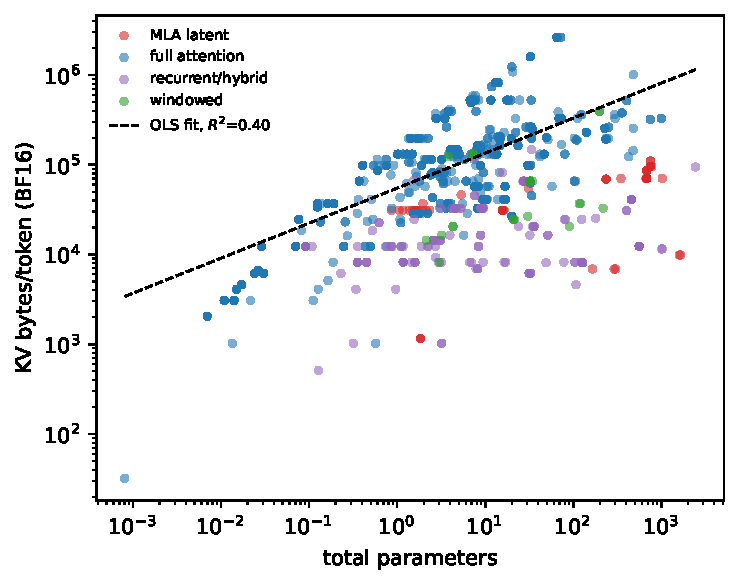
\includegraphics[width=.6\linewidth]{figures/fig2_kv_vs_params.pdf}
\caption{KV bytes per token against total parameters (log--log) with the OLS fit; color encodes attention class.}
\label{fig:kv-params}
\end{figure}

\begin{figure}[t]
\centering
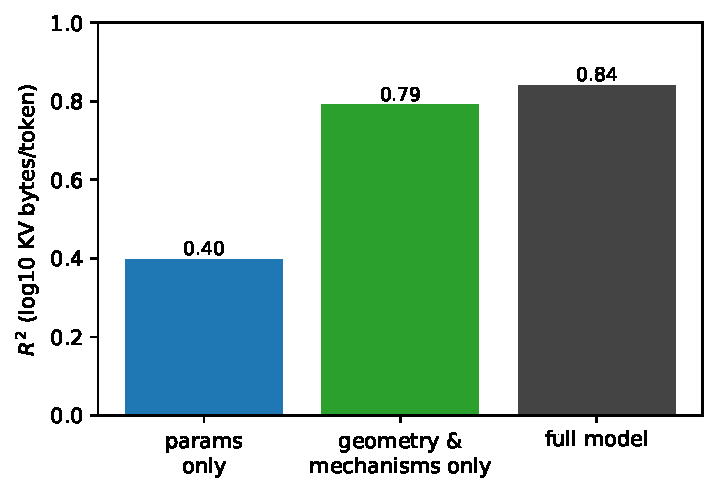
\includegraphics[width=.6\linewidth]{figures/fig3_mechanism.pdf}
\caption{Variance explained ($R^2$) of $\log_{10}$ KV bytes/token by parameter count alone,
by attention geometry and mechanisms alone, and by the full model. Parameter count is a weak
predictor compared with geometry.}
\label{fig:mechanism}
\end{figure}

Figure~\ref{fig:kv-params} regresses $\log_{10}$ KV bytes per token on $\log_{10}$ total parameters. The slope is \kvcParamsSlope{} with $R^{2}=\kvcParamsRsq$ (95\% CI \kvcParamsRsqLo--\kvcParamsRsqHi, 1000 bootstrap resamples), so H2 is \kvcHTwoVerdict{} by the pre-registered criterion ($R^{2}<0.5$): parameters alone leave most variance unexplained. Attention geometry alone---GQA ratio, head dimension, depth, window share, recurrent share, and the MLA and cross-layer-sharing indicators---predicts KV cost with $R^{2}=\kvcGeomRsq$; adding log parameters raises it to \kvcFullRsq{} (parameters alone: \kvcParRsq). The regression uses $N=\kvcRegN{}$ groups after excluding \kvcRegZeroKV{} zero-marginal-KV rows, whose asymptotic marginal cost is zero because every cache-bearing layer is windowed or recurrent.

% AUTO-GENERATED
\begin{table}[t]\centering\small
\caption{Standardized coefficients of the mechanism regression on $\log_{10}$ KV bytes/token.}\label{tab:mechanism}
\begin{tabular}{lrr}\toprule predictor & $\beta$ (std.) & VIF\\\midrule
total params ($\log_{10}$) & 4.928 & 7.3\\
GQA ratio ($\log(1+r)$) & 0.408 & 2.0\\
head dim & -0.419 & 2.3\\
depth ($\log(1+L)$) & 0.166 & 5.6\\
window layer share & 0.294 & 1.1\\
recurrent layer share & -0.082 & 1.1\\
MLA latent (0/1) & -0.214 & 1.2\\
cross-layer shared KV (0/1) & -0.237 & 1.0\\
\midrule
$N$ & \multicolumn{2}{r}{1930}\\
$R^2$ (full) & \multicolumn{2}{r}{0.841}\\
\bottomrule\end{tabular}\end{table}


Table~\ref{tab:mechanism} reports standardized coefficients. The architecture indicators act as designed: the MLA-latent indicator ($\beta=\kvcBetaLatent$) and cross-layer KV sharing ($\beta=\kvcBetaShared$) both lower predicted KV cost, consistent with latent compression \cite{deepseekai2024v2} and single-cache decoder designs \cite{sun2024yoco,wu2024cla}. Publisher behavior mirrors these mechanisms: Gemma~3 re-architected its attention layout specifically to curb KV growth by shortening local spans and thinning global layers \cite{gemmateam2025gemma3}. Two signs run against naive per-layer accounting---GQA ratio enters positively ($\beta=\kvcBetaGqa$) and head dimension negatively ($\beta=\kvcBetaHeadDim$), while window share ($\beta=\kvcBetaWindowShare$) and depth ($\beta=\kvcBetaDepth$) enter positively---because the coefficients are partial correlations conditioned on parameter count and depth, whose VIFs (\kvcVifParams{} and \kvcVifDepth, Table~\ref{tab:mechanism}) mark substantial collinearity. A model that spends its parameter budget on more layers must, at fixed KV-head width, buy KV with them. We therefore read the variance decomposition as the mechanism evidence, not the individual signs.

MoE models carry far less KV per total parameter, confirming H3 (\kvcHThreeVerdict). Median KV per $10^{9}$ parameters is \kvcMedKvppDense{} for dense models ($N=\kvcDenseN$) against \kvcMedKvppMoe{} for MoE models ($N=\kvcMoeN$): a ratio of \kvcHThreeRatio, far below the registered $0.5$ threshold (Mann--Whitney $p=\kvcMoeP$, rank-biserial \kvcMoeRB). Experts add parameters without adding per-token attention cache \cite{jiang2024mixtral,deepseekai2024v2}, and recent open families ship dense and MoE variants on the same attention stack \cite{yang2025qwen3}. Sizing serving hardware by total parameter count therefore overstates the memory cost of sparse models.

\subsection{RQ3: the KV-parity boundary moved, but not by orders of magnitude}
\label{sec:rq3}

\begin{figure}[t]
\centering
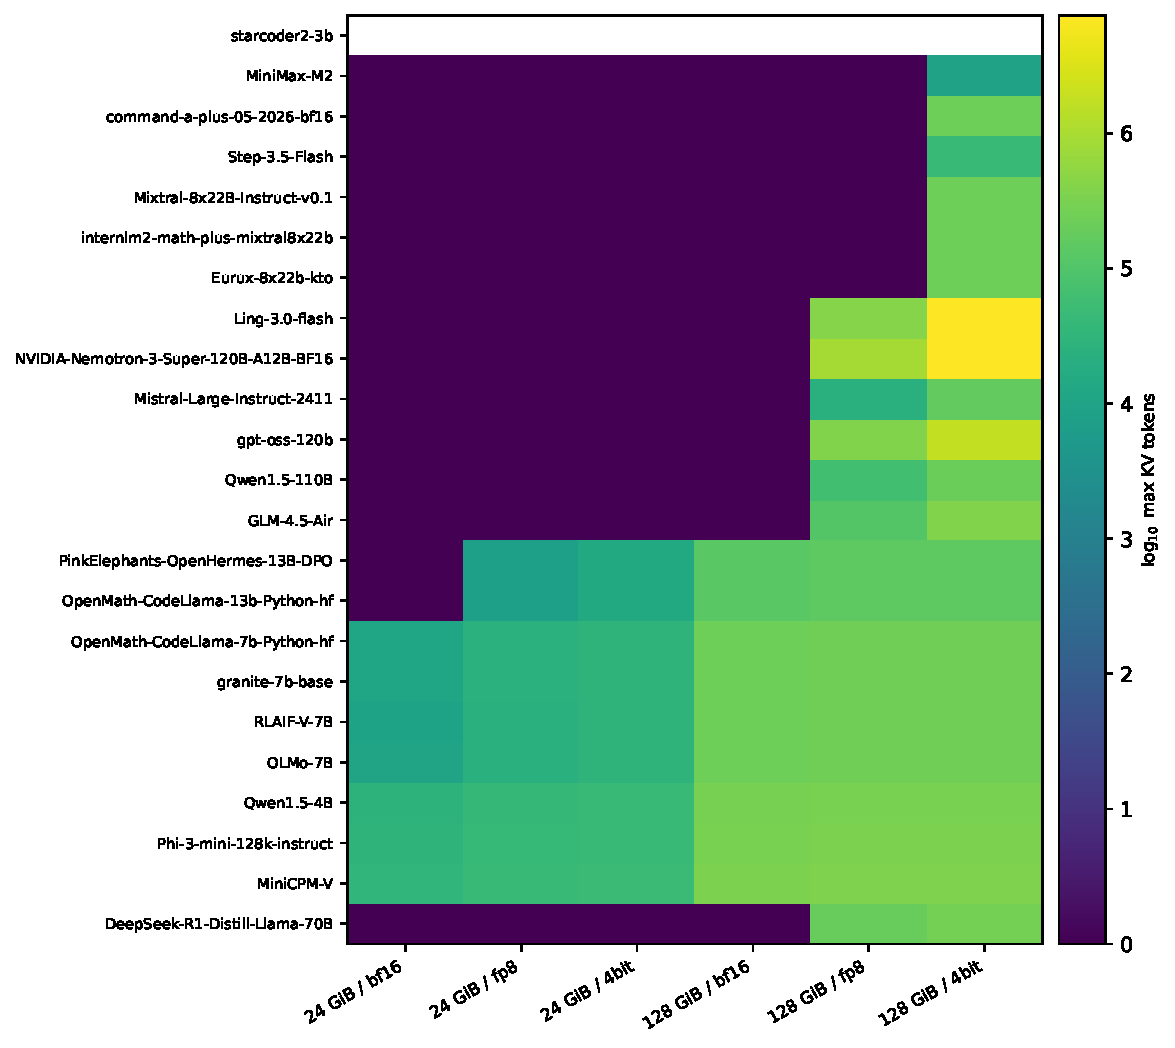
\includegraphics[width=.8\linewidth]{figures/fig4_capacity_heatmap.pdf}
\caption{Maximum total KV tokens (color: $\log_{10}$) across memory budgets and weight precisions, KV in BF16, 6\,GiB runtime overhead; rows follow the objective selection rule documented in the analysis code.}
\label{fig:capacity}
\end{figure}

% AUTO-GENERATED
\begin{table}[t]\centering\scriptsize\setlength{\tabcolsep}{3.5pt}
\caption{Maximum KV tokens at 6 GiB runtime overhead, KV in BF16; \lq--\rq{} means the weights alone exceed the budget, $\infty$ means the cache saturates (bounded window/state).}\label{tab:capacity}
\begin{tabular}{lrrrrrr}\toprule
model & 24/BF16 & 24/FP8 & 24/4b & 128/BF16 & 128/FP8 & 128/4b\\\midrule
starcoder2-3b & $\infty$ & $\infty$ & $\infty$ & $\infty$ & $\infty$ & $\infty$\\
MiniMax-M2 & -- & -- & -- & -- & -- & 9k\\
command-a-plus-05-2026-bf16 & -- & -- & -- & -- & -- & 230k\\
Step-3.5-Flash & -- & -- & -- & -- & -- & 47k\\
Mixtral-8x22B-Instruct-v0.1 & -- & -- & -- & -- & -- & 226k\\
internlm2-math-plus-mixtral8x22b & -- & -- & -- & -- & -- & 226k\\
Eurux-8x22b-kto & -- & -- & -- & -- & -- & 226k\\
Ling-3.0-flash & -- & -- & -- & -- & 431k & 7.3M\\
NVIDIA-Nemotron-3-Super-120B-A12B-BF16 & -- & -- & -- & -- & 891k & 7.5M\\
Mistral-Large-Instruct-2411 & -- & -- & -- & -- & 23k & 172k\\
gpt-oss-120b & -- & -- & -- & -- & 384k & 1.8M\\
Qwen1.5-110B & -- & -- & -- & -- & 60k & 209k\\
GLM-4.5-Air & -- & -- & -- & -- & 109k & 365k\\
PinkElephants-OpenHermes-13B-DPO & -- & 8k & 15k & 128k & 144k & 151k\\
OpenMath-CodeLlama-13b-Python-hf & -- & 8k & 15k & 128k & 144k & 151k\\
OpenMath-CodeLlama-7b-Python-hf & 11k & 24k & 30k & 224k & 237k & 243k\\
granite-7b-base & 11k & 24k & 30k & 224k & 237k & 243k\\
RLAIF-V-7B & 10k & 23k & 29k & 223k & 236k & 242k\\
OLMo-7B & 11k & 24k & 29k & 224k & 237k & 242k\\
Qwen1.5-4B & 28k & 38k & 42k & 301k & 310k & 314k\\
Phi-3-mini-128k-instruct & 30k & 39k & 44k & 314k & 323k & 328k\\
MiniCPM-V & 34k & 43k & 47k & 337k & 346k & 350k\\
DeepSeek-R1-Distill-Llama-70B & -- & -- & -- & -- & 184k & 279k\\
\bottomrule\end{tabular}\end{table}


We define the KV-parity context $T^{*}$ as the context length at which one sequence's KV bytes equal its BF16 weight bytes; beyond $T^{*}$ the cache, not the weights, dominates memory. Figure~\ref{fig:capacity} and Table~\ref{tab:capacity} give the capacity view under fixed budgets. Three regimes coexist. Small full-context models serve tens of thousands of KV tokens at 24\,GiB and hundreds of thousands at 128\,GiB. The largest recent open models enter the table only at 128\,GiB, several of them only once weights drop to 4-bit---\texttt{gpt-oss-120b} reaches 1.8M total KV tokens there---and \kvcInfeasibleBigModels{} census models exceed 128\,GiB on weights alone even at 4-bit. At the other extreme, \texttt{starcoder2-3b} never saturates: every layer is windowed, so its cache is bounded and total capacity is unlimited. How much precision buys depends on the weight share of the budget. \texttt{OLMo-7B} serves 11k tokens at 24\,GiB with BF16 weights and 24k with FP8 weights, because freed weight bytes flow straight into the KV pool; at 128\,GiB the same model gains little (224k versus 237k) because its budget is already KV-dominant. For the largest models, weight quantization \cite{frantar2022gptq} and KV quantization \cite{liu2024kivi,hooper2024kvquant} decide whether any cache fits at all. This is the regime PagedAttention was built for: KV memory, not parameters, limits batch size \cite{kwon2023paged}, and on unified-memory devices it decides how many long contexts coexist \cite{rajesh2025edgemem}.

\begin{figure}[t]
\centering
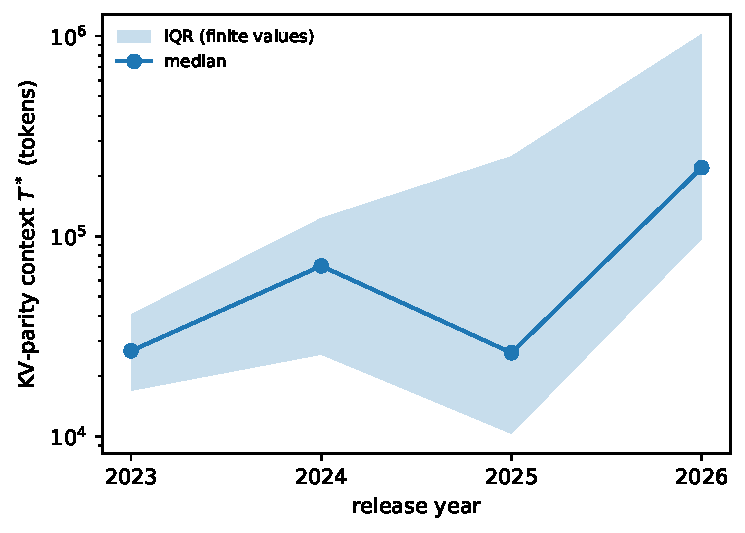
\includegraphics[width=.55\linewidth]{figures/fig5_parity_trend.pdf}
\caption{Median and IQR of finite KV-parity contexts $T^{*}$ by release year, log-scale $y$ axis.}
\label{fig:parity}
\end{figure}

The parity trend (Figure~\ref{fig:parity}) is the honest counterweight to the capacity headline. Median $T^{*}$ moved from \kvcParityMedTwentyThree{} tokens in 2023 to \kvcParityMedTwentyFour{} in 2024, fell back to \kvcParityMedTwentyFive{} in 2025---slightly below the 2023 median---and jumped to \kvcParityMedTwentySix{} in 2026. The share of models that are KV-dominant at 32k context ($T^{*}<32$k) fell from \kvcDominantShareTwentyThree\% in 2023 to \kvcDominantShareTwentySix\% in 2026, but not monotonically: it rebounded to \kvcDominantShareTwentyFive\% in 2025, the same small-model release-mix effect as in RQ1. A small and growing fraction of releases have no finite parity point at all---\kvcParityInfShareTwentyThree\% in 2023 versus \kvcParityInfShareTwentySix\% in 2026---because their caches saturate (fully windowed or recurrent). Against the pre-registered claim, H4 is \kvcHFourVerdict: pooled 2025--2026 median $T^{*}$ is only \kvcHFourRatio{}$\times$ the 2023 median, far from the registered $10\times$. The boundary did move, and context demand grew apace \cite{peng2023yarn}, so for the median 2025 release the cache still overtakes the weights at a context length near its 2023 position.

\subsection{RQ4: analytic accounting matches measured caches}
\label{sec:rq4}

\begin{figure}[t]
\centering
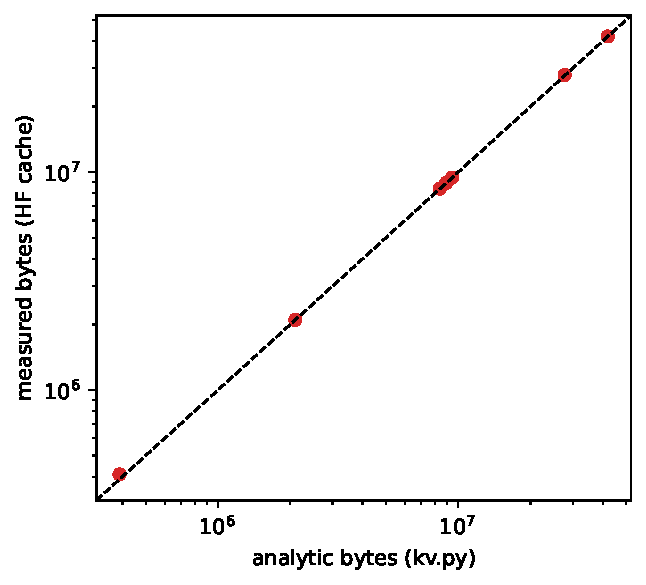
\includegraphics[width=.5\linewidth]{figures/fig6_validation.pdf}
\caption{Analytic (kv.py) versus measured HF cache bytes on reduced-depth random-init instances, log--log; the dashed line is equality.}
\label{fig:validation}
\end{figure}

% AUTO-GENERATED
\begin{table}[t]\centering\small
\caption{RQ4 validation: analytic (kv.py) vs measured HF cache bytes on reduced-depth random-init instances.}\label{tab:validation}
\begin{tabular}{llrrrl}\toprule model & class & analytic & measured & rel.err & note\\\midrule
phi-2 & mha & 41.94M & 41.94M & 0.000\% & MHA reference: 32 q/kv heads, head\_dim 80 (hidden 2560 / 32)\ldots\\
Qwen2.5-0.5B & gqa & 2.10M & 2.10M & 0.000\% & GQA reference: 14 q heads / 2 kv heads, head\_dim 64 (explici\ldots\\
starcoder2-3b & gqa+swa & 8.39M & 8.39M & 0.024\% & sliding-window GQA: all layers windowed, W=4096 (config slid\ldots\\
gpt-oss-20b & gqa+swa & 8.91M & 8.91M & 0.046\% & window+global hybrid (layer pattern [sliding, full], period \ldots\\
DeepSeek-V2-Lite & mla & 9.44M & 9.44M & 0.000\% & MLA: kv\_lora\_rank 512 + qk\_rope\_head\_dim 64; 2 layers kept =\ldots\\
granite-4.0-h-micro & hybrid-mamba & 27.73M & 27.89M & 0.565\% & hybrid mamba2+attention: attention at layer idx 5, 15, 25, 3\ldots\\
mamba-2.8b & mamba & 0.39M & 0.41M & 5.263\% & pure recurrent (Mamba-1 SSM); state is T-independent, T=512 \ldots\\
\bottomrule\end{tabular}\end{table}


The validation experiment instantiates reduced-depth, randomly initialized models from the snapshotted configs and measures the bytes of every cache tensor after prefill. It covers \kvcValRows{} models spanning \kvcValClasses{} attention classes (mha, gqa, windowed GQA hybrids, MLA, hybrid-Mamba, pure recurrent), and \kvcValWithin{} of the rows agree with the analytic accounting within 1\%, meeting the pre-registered success criteria (Figure~\ref{fig:validation}, Table~\ref{tab:validation}). Three implementation findings explain every nonzero gap. First, \texttt{transformers}~5.19 enforces sliding windows in the cache itself, not only in the attention mask: once a window saturates, the implementation truncates the stored tensor and retains one position fewer than the analytic $\min(T,W)$, which accounts for the small negative deviations on the two windowed probes. Second, the MLA implementation caches the compressed latent---the low-rank plus rope dimensions per token---and never materializes decompressed keys and values, so the theoretical latent accounting matches exactly \cite{deepseekai2024v2}. Third, recurrent layers pad their convolution state to the full kernel width, where the analytic model charges the theoretical minimum of stored inputs; this conv-state padding is the only deviation above 1\% (the pure-Mamba probe) and also explains the sub-1\% residual on the hybrid probe \cite{gu2023mamba}.
